\section{Distribution of the Utility Functions}
After finding the linear utility function corresponding to each user, we now move on to finding the distribution of the utility functions. Here, the input to our problem is a set of $N$ utility functions represented by their weight vectors, that is, a set of $N$ $d$-dimensional vectors. Based these $N$ utility functions, we want to find out from what distribution they most likely have been drawn. In this section, we propose two different approaches using clustering and density estimation to address the problem.

\subsection{Clustering Using Gaussian Mixture Model}
The main problem in finding the probability distribution of the utility functions is that there are users that attach different weights to different dimensions. For instance, in the hotel example, we might have some users that attach more value to the price compared to the location of the hotel and some other users vice versa, that is, the users consist of two general groups. Therefore, we expect to see a probability distribution that attaches higher probability to each of these two groups and lower probability elsewhere. Expressing such a probability distribution with a single probability density function is relatively hard. 

Instead, we can divide the users into groups and assign a probability distribution to each of the groups. This way, each group of users will contain users with similar characteristics, which makes it easer to assign a single probability distribution to each of the groups of the users. As a result we can use a mixture model to express the probability distribution of all the utility functions. Using such a model, we are reducing the problem of finding the distribution of all the utility functions to the problem of finding the distribution for the subsets of the utility functions. To obtain a distribution for all the utility functions, we furthermore, need to assign different weights to different groups of the utility functions. 

To be more specific, assume we have $k$ clusters of utility functions. Let $\phi_i$ be the probability density function of the $i$-th cluster. Then, we can write the final probability density function as $\phi(w) = \sum_{i = 1}^{k}\alpha_i \phi_i(w)$, where $\alpha_i$ is the weight attached to the $i$-th cluster. $\alpha_i$s must sum to 1 for this to be a valid probability density functions. Intuitively, $\alpha_i$ can be seen as the probability of an unknown observation falling into the cluster $i$. 

In order to use such a mixture model, we need to first find the $k$ clusters of the utility functions. Then, we need to find the values of $\alpha_i$s as well as the probability density function for each of the clusters.

First, let's discuss how we model the distribution of each of the clusters. The only information we have about each cluster is the observations from the distribution. We can treat these observation as random samples from our original distribution. So, from the sampled points, we want to find the probability distribution from which the points were sampled. 

Naturally, we can assume that the further away we go from the cluster, the probability of the points should decrease. This is because of our random sampling assumption and that if the probability was not less for points at distant locations from the cluster, there should  have been a point at those locations in the sample. Secondly, inside the cluster, we assume that as we go further towards the center of the cluster, the probability of the points should increase. However, this increase should be at a rate less than decrease rate outside the cluster. This is because when inside the cluster, moving towards the center means that we are moving away from some of the sample points while moving towards some other (at the other side of the cluster). We will discuss later how we calculate the center of a cluster or the distance of a point to a cluster, but to build our distribution, we use these two assumptions.  

A distribution that fits the above assumptions very well is a Gaussian distribution. We can assume that $\phi_i$ defined above is the probability density function of a normal distribution $\mathcal{N}(\mu_i, \sigma_i)$, where $\mu_i$ and $\sigma_i$ are the mean and standard deviation of the Gaussian distribution of the $i$-th cluster. Then, if $\mu_i$ is at the center of the cluster, the probability distribution will match our intuition perfectly. Furthermore, we can use the variance of the distribution to adjust it further. For instance, if we have a distribution that is not concentrated or dense, then we can assign a lager variance to it. On the other hand, we can assign lower variance to a cluster that is dense and concentrated around a center. With lower variance, the probability of a set of points being at a distance $x$ from the cluster would be lower than their probability with a higher variance.

With the Gaussian distribution assumption for each of the clusters, the only thing that remains is to find the parameters $\mu_i$ and $\sigma_i$ for each of the distributions and all the $\alpha_i$s to be able to create the final Gaussian mixture model. A method commonly used in the literature is Expectation Maximization \cite{ML}. Informally, this method first calculates the probability of each sample belonging to each of the clusters and then, based on this probability, tries to calculate the parameters of the distributions. It continues repeating the steps until there is no change in the parameters. After using the expectation maximization algorithm, we will be able to find a find the probability distribution of the utility functions, which was the aim of this paper. 

Although this approach provides a means for us to solve the problem, there are a few downsides in using it. Firstly, we need to know the number of clusters initially, which might not be possible in many situations. Furthermore, it assumes a Gaussian distribution on the utility functions in each of the clusters which is not necessarily valid. Moreover, there is no guarantee on the time complexity of the algorithm and the number of iterations it will take. 

\begin{figure*}[ht]
	\includegraphics[width=1\textwidth]{data.eps}
	\caption{Estimating non-linear utility functions}
\end{figure*}
\begin{figure*}[ht]
	\includegraphics[width=1\textwidth]{data2.eps}
	\caption{Estimating linear utility functions}
\end{figure*}
\subsection{Density Estimation}
To address the shortcomings of the Gaussian mixture model, we propose another method to find the probability distribution of the utility functions. The discussion here falls under the area of kernel density estimation in statistics. 

As mentioned above, we can see the problem of finding the distribution of utility functions as the problem of estimating the probability density function of a random variable based on a finite sample of observations of the values of the random variable. Note that the only information we have about the original distribution is the samples drawn from it. So, to estimate the probability of a set of points, we can only look at how similar the points are to the sampled data. That is, the probability of a set of points, $X$, (we use a set of points because the probability of any specific point is zero in a continuous distribution) depends on how \textit{close} this set of points is to the sample points. Thus, we can estimate the original distribution using a \textit{distance} measure.

One way to do this is to define a probability density function based on the Euclidean distance between a point and the sample points. To be more specific, we can write the probability density function as 
\begin{equation*}
f(x) = \frac{1}{N}\sum_{i = 0}^{N}K(x - xi)	
\end{equation*}

where $K(y)$ is called a kernel function. The kernel function measures how the distance between $x$ and a sample point affects the probability distribution, and it should add to 1 over all possible values of $x$. $K(y)$ itself can be seen as a probability density function that measures the probability of the difference of a point from a specific sample point being $y$. In other words, we can see $K(x - x_i)$ as the probability distribution function if there is only one sample point $x_i$ is observed. This way, we can see the distribution of the utility functions as a mixture model with $N$ components where each component is given the weight $\frac{1}{N}$. Then, the problem that remains is that what should the kernel function $K(y)$ be. 

There are different kernel functions that are commonly used. One of them is a Gaussian function. We propose the use of a Gaussian kernel for the same reason discussed above regarding the use of the Gaussian mixture model. That is, we expect the probability to be to be larger for the points closer to a sample point and smaller for the points  further away from the sample point, a property that is satisfied by a Gaussian kernel. Furthermore, the kernel does not impose any restriction on the range of values of $x$, which allows for continuous derivatives unlike, for instance, Epanechnikov kernel. This property can be used for clustering the data based on the probability density function. 

Another point to note is the co-variance of the Gaussian distribution. The co-variance  controls how much effect moving away from a single sample point has on the probability. The smaller the co-variance values, existence of a sample point will affect the points further away from the sample point much less. To evaluate a suitability of a co-variance matrix, a standard method is to use \textit{mean integrated squared error}. For our implementation, we use \textit{Silverman's rule of thumb} which uses the co-variance matrix, $\Sigma$ as $\Sigma_{ii} = \frac{4\sigma_i}{N(d+2)}^{(\frac{2}{d+4})}$ and $\Sigma_{ij, i \neq j} = 0$ where $\Sigma_{ij}$ is the element in the $i$-th row and $j$-th column of the co-variance matrix and $\sigma_i^2$ is the variance of the $i$-th dimension of the sample points (see \cite{silverman} for details and proofs). Note that it can be proven that with such a Gaussian kernel, as $N$ approaches infinity, the estimated distribution will approach the true distribution of the random variable. That is, our estimation becomes more accurate as the number of points increase.

Using such a Gaussian kernel, we can write the final probability density functions as 
\begin{equation*}
f(x) = \frac{1}{N}\sum_{i = 0}^{N}\frac{e^{(-\frac{1}{2}(x - x_i)^T\Sigma^{-1}(x - x_i))}}{\sqrt{\left\vert2\pi\Sigma\right\vert}}.
\end{equation*}

Therefore, by integrating this probability density function over any set of values, we will be able to find the probability of having a utility function among those values. For instance, in the hotel example, we can find the probability of a user giving more than 50 percent value to price by calculating $\int_{x_1>0.5}f(x_1, x_2, x_3)dx_1dx_2dx_3$ where $x_1$ denotes price, $x_2$ location and $x_3$ size. We can similarly calculate the probability of a user attaching more than 50 percent value to location and compare the two.

Using kernel density estimation or the Gaussian Mixture model to calculate the probability of a set of utility functions will involve the calculation of $N$ or $k$ number of $d$ dimensional integrals. We can use Monte Carlo methods to approximate the value of such an integral to a desired precision at the trade off of the running time. In general, such algorithms will run in $O(\alpha Nd)$ where the larger $\alpha$ is, the lower the error estimate of the calculations will be, while the error estimate does not depend on the dimensionality of the data. 

Furthermore, sampling can be easily done from either of the proposed approaches. To sample a point from a Gaussian mixture model we first select one of the components, based on the weight each component has, and then sample the Gaussian distribution of the component. In case of kernel density estimation, we follow the same procedure, except that here the components of the mixture model are comprised of the original sample points we had, and each component is equally likely to be selected (the weight given to each component is $\frac{1}{N}$). Similarly, after selecting a component, we draw a sample from its Gaussian distribution. 

Finally, note that the kernel density estimation provides a nonparametric modeling of the data. As such, there are no parameters in the model that need to be learned from a training dataset. This means that to use such an estimation, we can only use its closed form formula for the calculation and no other processing step is needed. This is while for a Gaussian mixture model, we need to run the expectation maximization algorithm to find the parameters of the model. However, to calculate any probability based on the kernel density estimation we need to calculate $N$ integrals, while this value is reduced to $k$ in the Gaussian mixture model, where $k$ is expected to be orders of magnitude smaller than $N$. Moreover, Gaussian mixture model provides clustering of the data as well, although it requires the number of the clusters in advance. Kernel density estimation, on the other hand, does not provide any clustering of the utility functions. 






